\documentclass[
  journal=largetwo,
  manuscript=article-type,
  year=2023,
  volume=1,
]{iitp-journal}

\usepackage{amsmath}
\usepackage[nopatch]{microtype}
\usepackage{booktabs}
\usepackage{minted}
\usepackage{listings}
\usepackage{hyperref}
\usepackage[backend=biber, sorting=none]{biblatex}

\title{Generation of Terrain Map using Autonomous Quadcopter}

\author{Kartikay Gupta}
% \affiliation{Second Division, Organization, City, Pincode, State, Country}
% \alsoaffiliation{Joint first authors}

\author{Shresth Verma}
% \affiliation{Third Division, Organization, City, Pincode, State, Country}

\author{Nitesh Srivastava}
% \affiliation{First Division, Organization, City, Pincode, State, Country}
% \email[F. Author]{first.author@address.edu}

\author{Prateek Kumar}
% \affiliation{Fourth Division, Organization, City, Pincode, State, Country}

\author{Deepanshu Chaudhary}
% \affiliation{Fifth Division, Organization, City, Pincode, State, Country}

\bibliography{example}

\keywords{Quadcopter, Image Stitching, OpenCV} %% First letter not capped

\begin{document}

\begin{abstract}
In this paper, we present a method for generating panoramic images of a region using an automated Parrot AR 2.0 Quad-copter drone. The drone travels in a snake-like pattern over the region, capturing images, and sending them to a server computer. The server computer then applies image stitching algorithms to generate the panorama. Our approach provides a low-cost, flexible, and fully automated solution for generating panoramic images of a region. We discuss the challenges and solutions in the design and implementation of the system, as well as the results of testing the system in a real-world scenario.
\end{abstract}

% \noindent Lorem ipsum dolor sit amet, consectetur adipiscing elit, sed do eiusmod tempor incididunt ut labore et dolore magna aliqua. 

\section{1. Introduction}
In recent years, drones have become increasingly popular for aerial mapping and surveying. They are a cost-effective and flexible alternative to satellite imaging for generating panoramic images. They can provide high-resolution, real-time images that can be captured in areas where satellites may not be able to reach. Additionally, drones allow for customizable flight paths, allowing for specific images to be captured for a given project. These benefits make drone-based panoramic image capture a compelling choice for many applications.

In this paper, we consider the problem of generating a panoramic image of a region using a fully automated Parrot AR 2.0 Quad-copter. Figure 1 shows AR 2.0 drone used in this study. 

\begin{figure}[hbt!]
\centering
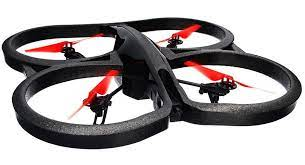
\includegraphics[width=0.75\linewidth]{AR-2.0-quadcopter.jpeg}
\caption{Parrot AR Drone 2.0}
\label{fig_sim}
\end{figure}

Previous approaches have used mechanical control or some constraints on image sequence in order to map the region. In this work, we present the design and development of an autonomous drone for mapping applications. The Parrot AR 2.0 Quadcopter is a lightweight drone with a weight of approximately 400 grams. It has a limited connectivity range of 50 meters, meaning that the controller must be within 50 meters of the drone in order to maintain control. The drone is equipped with two cameras: a frontal camera with 720p resolution, and a QVGA vertical camera. These cameras allow the drone to capture high-quality images and video, making it well-suited for aerial photography and mapping applications. It has a built-in WiFi network that can be used to share video and images in real-time, and it also has a number of safety features, such as automatic return-to-home, to ensure that the drone can be safely recovered in the event of a problem and GPS stabilization, allowing it to fly in a stable manner even in windy conditions.

The drone can be programmed to fly over a specific area and capture video, which it sends to the server computer as a real-time data. The server then performs image stitching techniques to generate the map of the region. This map can be used for various purposes such as surveying, agriculture, and environmental monitoring. In addition, we discuss the challenges and solutions in the design and development of the drone, as well as the results of testing the drone in a real-world scenario.
% The drone is equipped with a camera and onboard computer to capture video and process it into a map of the area flown over. 
% By default, this template uses \texttt{biblatex} and adopts the Chicago referencing style. If you are using this template on Overleaf, Overleaf's build tool will automatically run \texttt{pdflatex} and \texttt{biber}. If you are compiling this template on your own local \LaTeX{} installation, please execute the following commands:
% \begin{enumerate}
%     \item \verb|pdflatex sample|
%     \item \verb|biber sample|
%     \item \verb|pdflatex sample|
%     \item \verb|pdflatex sample|
% \end{enumerate}

% Some journals e.g.~\texttt{journal=aog|jog|pasa}
% \\require Bib\TeX{}. For such journals, you will need to
% \begin{itemize}
%     \item delete the existing \verb|\addbibresource{example.bib}|;
%     \item change the existing \verb|\printbibliography| to be\\
%     \verb|\bibliography{example}| instead.
% \end{itemize} 

% Overleaf will run \texttt{pdflatex} and \texttt{bibtex} automatically as needed. But if you had \emph{first} compiled using another \texttt{journal} option that adopts \texttt{biblatex}, and \emph{then} change the \texttt{journal} option to one that adopts Bib\TeX{}, you may get some compile error messages instead. In this case you will need to do a `Recompile from scratch'; see \url{https://www.overleaf.com/learn/how-to/Clearing_the_cache}.

% On a local \LaTeX{} installation, you would need to run these steps instead:
% \begin{enumerate}
%     \item Delete \texttt{sample.aux}, \texttt{sample.bbl} if these files from a previous compile using \texttt{biber} still exist.
%     \item \verb|pdflatex sample|
%     \item \verb|bibtex sample|
%     \item \verb|pdflatex sample|
%     \item \verb|pdflatex sample|
% \end{enumerate}

% Lorem ipsum dolor sit amet, consectetur adipiscing elit, sed do eiusmod tempor incididunt ut labore et dolore magna aliqua. 

% Lorem ipsum dolor sit amet, consectetur adipiscing elit, sed do eiusmod tempor incididunt ut labore et dolore magna aliqua. Lorem ipsum dolor sit amet, consectetur adipiscing elit, sed do eiusmod tempor incididunt ut labore et dolore magna aliqua. 

\section{2. Literature Review}
\subsection{2.1 Path-Tracking control of quadcopter}
Autonomous control of drones has been an active area of research for several years. With advancements in drone technology and increase in their applications, the need for efficient and reliable control systems has become imperative. In the recent past, a number of studies have been carried out to address the issue of autonomous drone control. Some of these works have used conventional control systems such as Proportional-Integral-Derivative (PID) control \cite{1} and Model Predictive Control (MPC) \cite{2}, while others have utilized more advanced methods such as reinforcement learning and neural networks \cite{3}.

Nodejs, an open-source and cross-platform JavaScript runtime environment, has been widely used in recent years for various applications, including web development and Internet of Things (IoT). However, its use in the field of autonomous drone control is relatively limited. There \cite{4} have been a few studies that have utilized Nodejs for drone control, but they have mostly focused on controlling the drone in a specific environment or task.

The aim of our research is to contribute to the field of autonomous drone control by utilizing Nodejs to control a quadcopter for the purpose of mapping a region. Our work builds upon the existing literature by combining the capabilities of Nodejs with state-of-the-art image stitching algorithms, such as ORB and SIFT, to generate an accurate and comprehensive terrain map.

In summary, our literature review highlights the need for autonomous drone control systems and the limited use of Nodejs in this field. Our research fills a gap in the literature by utilizing Nodejs to control a quadcopter for the purpose of mapping a region, which has not been done before.

\subsection{2.2 Terrain Map generation}
Terrain mapping using computer vision algorithms and tools is a rapidly growing area of research in the field of geospatial analysis. In this work, we have used Python OpenCV stitcher class for mapping purposes.

Image stitching can be defined as the process of combining an arbitrary number of images with unified perspective by detecting the overlapping areas, so the images are aligned and blended with seamless edges .Fundamental Concepts in Image Stitching can be found in \cite{5}. Earlier techniques minimized pixel-to-pixel dissimilarities, but the recent algorithms work by extracting a set of feature points and then matching them. One early attempt to find these corners was done by Chris Harris, now called the Harris Corner Detector Method. However, their major disadvantage was that these features were just Rotation Invariant and not Scale Invariant. Later, D. Lowe et al. came up with a breakthrough SIFT algorithm in \cite{6}. The SIFT algorithm has 4 basic steps. The first is to estimate a scale space extrema using the Difference of Gaussian (DoG). Secondly, a key point localization where the key point candidates are localized and refined by eliminating the low contrast points. Thirdly, a key point orientation assignment based on local image gradient and lastly a descriptor generator to compute the local image descriptor for each key point based on image gradient magnitude and orientation.

We have used OpenCV stitcher class for Image Stitching Purpose. It uses ORB algorithm for Image Stitching and derives its primary motivation from SIFT algorithm. It was put forward by Ethan Rublee et al. in \cite{7}. ORB is a fusion of the FAST key point detector and BRIEF descriptor with some 
modifications. Initially, to determine the key points, it uses FAST. Then a Harris corner measure is applied to find the top N points. FAST does not compute the orientation and is a rotation variant. It computes the intensity-weighted centroid of the patch with a located corner at centre. The direction of the vector from this corner point to the centroid gives the orientation. Moments are computed to improve the rotation invariance. The descriptor BRIEF poorly performs if there is an in-plane rotation. In ORB, a rotation matrix is computed using the orientation of the patch and then the BRIEF descriptors are steered according to the orientation. 

\subsection{2.3 Gaps}
In our research paper, we aim to address two significant gaps in the field of terrain map generation using a drone. Firstly, while a considerable amount of research has been done in the area of image stitching using drones, most of these studies have relied on manually controlled drones \cite{8}. Our research attempts to fill this gap by developing a quadcopter autonomously controlled using NodeJS. This innovative aspect of our research provides a more robust and scalable solution for terrain map generation.

Secondly, we noticed a lack of comprehensive data collection using a quadcopter while implementing image stitching algorithms \cite{9}. To address this gap, we have incorporated a Ublox sensor that provides reliable and high-quality GPS data, such as latitude, longitude, and altitude. This data can significantly enhance the accuracy and precision of the terrain map generation process. In our study, we have used ORB-based image stitching algorithms comparable to traditional algorithms like SIFT and SURF in terms of accuracy and precision. Our use of ORB and our implementation of image stitching using Java BoofCV and OpenCV make our approach unique and a valuable contribution to the field of terrain map generation.

\section{3. Problem Statement}

The objective of this study is to develop a fully automated quadcopter capable of mapping a given region. The quadcopter collects image data using its HD 720p frontal camera and QVGA vertical camera and simultaneously obtains GPS coordinates using an Arduino Nano connected to U-blox GPS and NRF24l01 (Wi-Fi module). The drone is autonomously controlled using NodeJS, and the images are stitched to generate a terrain map using the stitcher class of Python OpenCV.

% \textbf{Given:} With the help of various sensors available in the Parrot AR Drone - 3-axis Accelerometer and 3-axis Magnetometer, Ultrasound Sensor, and 3-axis Gyroscope, we were able to obtain Roll, Pitch, Yaw angles, and rotation matrix. Also, the drone has 2 inbuilt cameras: HD 720p frontal camera and QVGA vertical camera, which enabled us to capture images at each instant. To get the GPS coordinates associated with each image, we mounted an Arduino Nano connected to U-blox GPS and NRF24l01 (Wi-Fi module) on the drone to transmit GPS data to our console in real-time.
% \\
% \\
% \textbf{To determine:} Our aim is to create a 2D map of a rectangular area by stitching the images transmitted by the drone and storing sensor and GPS data associated with each image.

% %%% Numbered equation
% \begin{equation}
% \begin{aligned}\label{eq:first}
% \frac{\partial u(t,x)}{\partial t} = Au(t,x) \left(1-\frac{u(t,x)}{K}\right)
%  -B\frac{u(t-\tau,x) w(t,x)}{1+Eu(t-\tau,x)},\\
% \frac{\partial w(t,x)}{\partial t} =\delta \frac{\partial^2w(t,x)}{\partial x^2}-Cw(t,x)
% +D\frac{u(t-\tau,x)w(t,x)}{1+Eu(t-\tau,x)},
% \end{aligned}
% \end{equation}

%  Lorem ipsum dolor sit amet, consectetur adipiscing elit, sed do eiusmod tempor incididunt ut labore et dolore magna aliqua. Lorem ipsum dolor sit amet, consectetur adipiscing elit, sed do eiusmod tempor incididunt ut labore et dolore magna aliqua. Lorem ipsum dolor sit amet, consectetur adipiscing elit, sed do eiusmod tempor incididunt ut labore et dolore magna aliqua. 

% \begin{align}\label{eq:another}
% \begin{split}
% \frac{dU}{dt} &=\alpha U(t)(\gamma -U(t))-\frac{U(t-\tau)W(t)}{1+U(t-\tau)},\\
% \frac{dW}{dt} &=-W(t)+\beta\frac{U(t-\tau)W(t)}{1+U(t-\tau)}.
% \end{split}
% \end{align}


% %%%% Unnumbered equation
% \begin{align*}
% &\frac{\partial(F_1,F_2)}{\partial(c,\omega)}_{(c_0,\omega_0)} = \left|
% \begin{array}{ll}
% \frac{\partial F_1}{\partial c} &\frac{\partial F_1}{\partial \omega} \\\noalign{\vskip3pt}
% \frac{\partial F_2}{\partial c}&\frac{\partial F_2}{\partial \omega}
% \end{array}\right|_{(c_0,\omega_0)}\\
% &\quad=-4c_0q\omega_0 -4c_0\omega_0p^2 =-4c_0\omega_0(q+p^2)>0.
% \end{align*}

\section{4. Overview of Approach}
\subsection{4.1 Sensor Integration into the quadcopter platform}
To access the images and sensor data captured by the AR drone, including the Roll, Pitch, and Yaw angles, Rotation Matrix, and Altitude, the console was connected to the drone via its Wi-Fi. Additionally, a U-blox GPS module was installed on the drone to capture GPS information. The U-blox GPS module was selected due to its high accuracy, wide connectivity, compact size and high sensitivity. The GPS module was connected to an Arduino Nano, which transmitted the GPS data in real time to the console using the NRF24l01 wireless module.

The use of the NRF24l01 module was motivated by its low power consumption, high data transfer rate, and small form factor. These advantages make it an ideal choice for applications that require real-time data transfer and power efficiency.

The images and sensor data captured by the AR drone were transmitted via its Wi-Fi. In contrast, the GPS coordinates corresponding to each image were transmitted by the Arduino Nano using the NRF24l01 module. This setup allowed for the seamless transmission of images as well as sensor data, ensuring that all relevant information was captured and transmitted in real-time. The console received GPS data by connecting it to Arduino UNO using NRF24l01 module.

\subsection{4.2 Autonomous Flight}
The drone was equipped with an in-built app for live streaming and controlling the device, but in order to move a drone autonomously and capture images along a specified path, we utilized a NodeJS library. This library provided us with the ability to program a specific path for the drone to follow, ensuring that the drone moved in a precise and controlled manner. To ensure the safety of the drone and its surroundings, a fail-safe mechanism was also incorporated into the system, which automatically triggered the drone to land in the event of any emergency or unexpected situation. This added an extra layer of security and peace of mind to the entire operation.

\subsection{4.3 Data Acquisition}
The AR drone captured images at a frequency of 7-8 per second and transmitted them to the console through WiFi in PNG format. Along with each image, the accompanying sensor and GPS data were recorded and saved in a JSON file format on our local system for easy access and analysis.

\subsection{4.4 Post-processing to generate 2D map}
The image stitching process plays a crucial role in generating the terrain map using a quadcopter. Our approach towards image stitching uses the stitcher class provided by Python OpenCV. The stitcher class integrates the ORB (Oriented FAST and Rotated BRIEF) algorithm for feature generation and image stitching.

The ORB algorithm is a fast and efficient alternative to traditionally used SIFT (Scale-Invariant Feature Transform) and SURF (Speeded-Up Robust Features) algorithms. ORB detects and describes local features in the images and then uses them to stitch the images together.

In our approach, the images captured by the quadcopter's 720p frontal camera and QVGA vertical camera are sent to the stitcher class. The stitcher class then applies the ORB algorithm to detect and describe local features in the images and stitch them together to form a panoramic view of the region.

\section{Sensor Integration into the quadcopter platform}
The drone is equipped with the following sensors as standard
\begin{itemize}
    \item 3-axis accelerometer (± 50 mg precision)
    \item 3-axis gyroscope (2000°/second precision)
    \item Pressure sensor (± 10 Pa precision / 31.5" (80 cm) at sea level)
    \item 3-axis magnetometer (6° precision)
    \item Ultrasound ground altitude measurement sensors (effective up to 19.7' (6 m) above the ground)
    \item Dynamic wind estimation sensor
    \item Built-in 3D compass
\end{itemize}
The included sensors enabled us to gather images and navigation information. Additional sensors were installed to acquire GPS data, the schematics of which are depicted below. Schematic for the sensors mounted on the drone to transmit GPS data can be clearly seen in Figure~\ref{fig:transmitter}. 
\begin{figure}
    \centering
    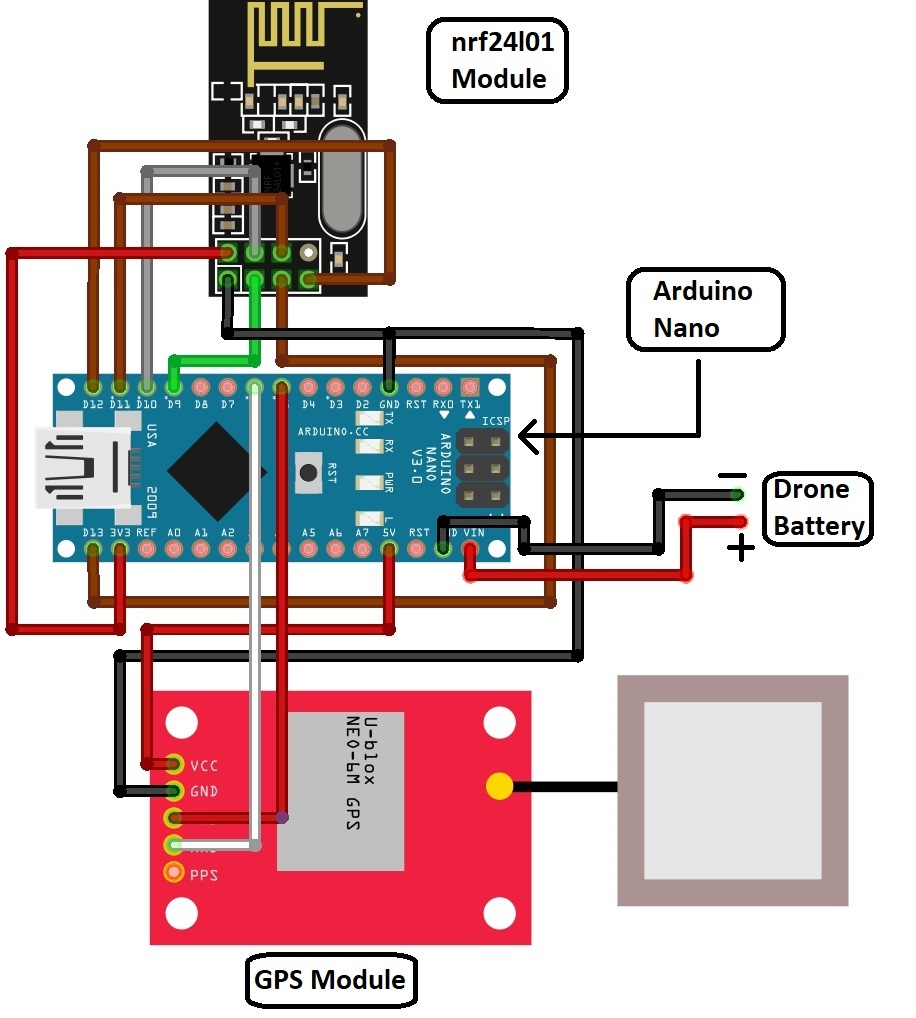
\includegraphics[width=0.7\textwidth]{Transmitter_circuit.jpg}
    \caption{Transmitter mounted on the drone}
    \label{fig:transmitter}
\end{figure}
\\
\\
Figure~\ref{fig:receiver} shown below is a schematic diagram for Arduino UNO and NRF module connected to the console for receiving data. 
\begin{figure}[h]
    \centering
    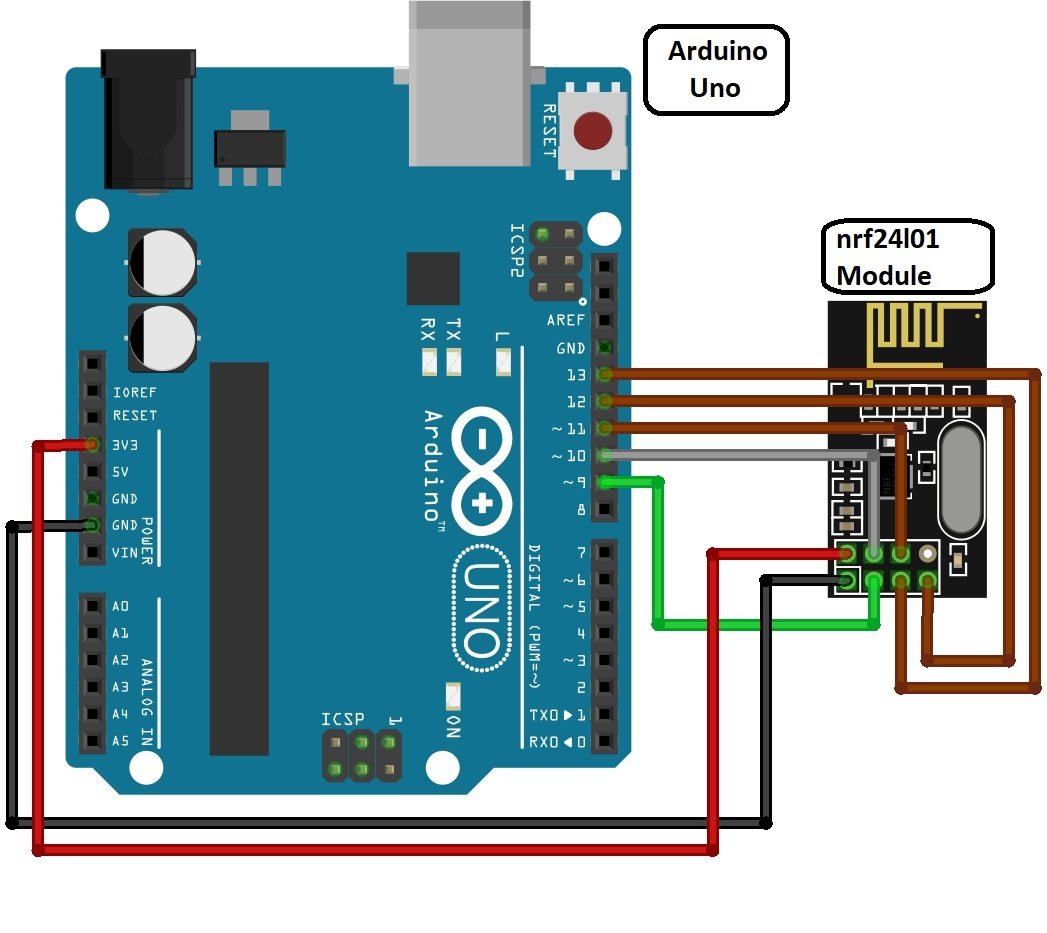
\includegraphics[width=0.7\textwidth]{Receiver_circuit.jpg}
    \caption{Receiver Circuit attached to console}
    \label{fig:receiver}
\end{figure}

\section{Autonomous Flight}
To have the drone operate independently, we utilized a NodeJS library and programmed a specific route similar to Figure~\ref{fig_path}.
% \\
Sample code for setting a path for drone:
\begin{minted}[breaklines=true]{javascript}
var arDrone = require('ar-drone');
var client  = arDrone.createClient();
// takeoff
client.takeoff();
client
.after(5000, function () {
    //move upwards
    this.up(0.4);
})
.after(14000, function () {
    this.stop();
    //move front
    this.front(0.1);
})
.after(12000, function () {
    this.stop();
    //move right
    this.right(0.1);
})
.after(3000, function () {
    this.stop();
    //move back
    this.back(0.1);
})
.after(11000, function () {
    this.stop();
    //move left
    this.left(0.1);
})
.after(2000, function () {
    this.stop();
    //land
    this.land();
});
\end{minted}
For more insight into the code, refer to  \href{https://github.com/KartuzGupta/Parrot-AR-Drone/blob/main/README.md}{this}.

\begin{figure}
    \centering
    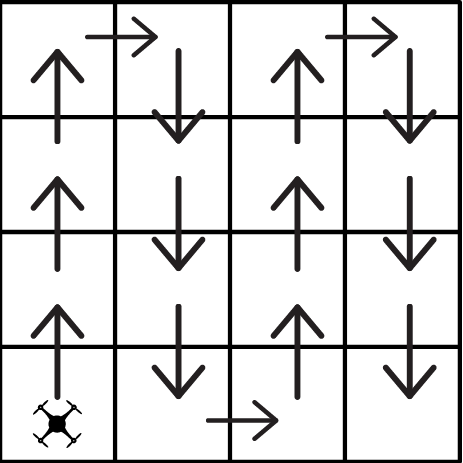
\includegraphics[width=0.6\linewidth]{path.png}
    \caption{Expected trajectory of drone}
    \label{fig_path}
\end{figure}

\section{Data Acquisition}
To access sensor data acquired by the drone, the console needed to be connected to the drone's wifi and the following codes were executed:
\begin{minted}[breaklines=true]{javascript}
// To access navigation data: Roll, Pitch & Yaw angles, Altitude, Rotation matrix. GPS data was also read simultaneously and stored in JSON format.
var arDrone = require('ar-drone');
var client = arDrone.createClient();
var start = process.hrtime();

client.on('navdata', (data)=>{
//Handle drone data processing here...
fs.readFile(`nav.json`, function(err, prev){
//reading GPS data
fs.readFile("GPS.txt", 'utf-8', function (err, gpstxt){
  if (err) throw err;
  if (data.hasOwnProperty('demo')) {
    // current time
    var current = process.hrtime(start);
    // GPS data in txt file is in format 'latitude,longitude,altitude'
    var gps = gpstxt.toString().split(',');
    var time = current[0];
    var dat = JSON.parse(prev);
    // saving data in JSON format corresponding to time
    dat[time]['drone'] = data;
    dat[time]['latitude'] = gps[0];
    dat[time]['longitude'] = gps[1];
    dat[time]['altitude'] = gps[2];
    // writing data to JSON file
    fs.writeFile(`nav.json`, JSON.stringify(dat),err=>{
      if (err) throw err;
    });
  }
});
});

\end{minted}
% \\
Sample data stored in JSON file
\begin{minted}{javascript}
//Sample navigation data
{"1":{
  drone: {
    header: 1432778632,
    demo: {
      controlState: 'CTRL_LANDED',
      flyState: 'FLYING_OK',
      batteryPercentage: 90,
      rotation: {
        frontBack: -0.616,
        pitch: -0.616,
        theta: -0.616,
        y: -0.616,
        leftRight: 0.659,
        roll: 0.659,
        phi: 0.659,
        x: 0.659,
        clockwise: 30.32,
        yaw: 30.32,
        psi: 30.32,
        z: 30.32
      },
      "altitude":1.136,
      drone: { camera: { {
          rotation: {
            m11: 0.8631653785705566,
            m12: -0.5049092769622803,
            m13: -0.003481418127194047,
            m21: 0.504806637763977,
            m22: 0.863095760345459,
            m23: -0.015362740494310856,
            m31: 0.010761587880551815,
            m32: 0.011503142304718494,
            m33: 0.9998759031295776
          },
          translation: { x: 0, y: 0, z: -234 }
        } } }
    },
  },
  longitude: '25.54128074',
  latitude: '84.85104370',
  altitude: '57'
}
}
\end{minted}
For more information regarding navigation data refer to \href{https://github.com/felixge/node-ar-drone/blob/master/docs/NavData.md}{this}.
\\
\\
The following code was used to store images captured by the drone in .png format
\begin{minted}[breaklines=true]{javascript}
// storing images captured by drone
var arDrone = require('ar-drone');
var client = arDrone.createClient();
var fs = require('fs');
//start time
var start = process.hrtime();

var pngStream = client.getPngStream();
pngStream
.on('error', console.log)
.on('data', function(pngBuffer) {
    // get current time
    var current = process.hrtime(start);
    // saving images
    fs.writeFile(`images/frame` + current[0] + '.png', pngBuffer, function(err) {
        if (err) {
            console.log('Error saving PNG: ' + err);
        }
    });
});

\end{minted}

The following codes were uploaded to Arduino for transmission and receiving GPS data.
\begin{minted}[breaklines=true]{arduino}
//Transmitter
\end{minted}

\begin{minted}[breaklines=true]{arduino}
//Receiver
\end{minted}

\section{Post-processing to generate 2D map}
ORB is basically a fusion of FAST keypoint detector and BRIEF descriptor with many modifications to enhance the performance. First it use FAST to find keypoints, then apply Harris corner measure to find top N points among them. It also use pyramid to produce multiscale features. But one problem is that, FAST doesn't compute the orientation. So what about rotation invariance? The authors came up with following modifications.

It computes the intensity-weighted centroid of the patch with located corner at center. The direction of the vector from this corner point to centroid gives the orientation. To improve the rotation invariance, moments are computed with x and y which should be in a circular region of radius r, where r is the size of the patch.

Now for descriptors, ORB use BRIEF descriptors. But we have already seen that BRIEF performs poorly with rotation. So ORB does "steer" BRIEF according to the orientation of keypoints. For any feature set of n binary tests at location (xi,yi), define a 2×n matrix, S which contains the coordinates of these pixels. Then using the orientation of patch, $\theta$, its rotation matrix is found and rotates the S to get steered(rotated) version S$\theta$.

ORB discretize the angle to increments of 2$\pi$/30 (12 degrees), and construct a lookup table of precomputed BRIEF patterns. As long as the keypoint orientation $\theta$ is consistent across views, the correct set of points S$\theta$ will be used to compute its descriptor.

BRIEF has an important property that each bit feature has a large variance and a mean near 0.5. But once it is oriented along keypoint direction, it loses this property and become more distributed. High variance makes a feature more discriminative, since it responds differentially to inputs. Another desirable property is to have the tests uncorrelated, since then each test will contribute to the result. To resolve all these, ORB runs a greedy search among all possible binary tests to find the ones that have both high variance and means close to 0.5, as well as being uncorrelated. The result is called rBRIEF.

For descriptor matching, multi-probe LSH which improves on the traditional LSH, is used. The paper says ORB is much faster than SURF and SIFT and ORB descriptor works better than SURF. ORB is a good choice in low-power devices for panorama stitching etc.

\section{Results and Discussion}

The output for a single-column figure is in Figure~\ref{fig_sim}.  Lorem ipsum dolor sit amet, consectetur adipiscing elit, sed do eiusmod tempor incididunt ut labore et dolore magna aliqua. Lorem ipsum dolor sit amet, consectetur adipiscing elit, sed do eiusmod tempor incididunt ut labore et dolore magna aliqua. Lorem ipsum dolor sit amet, consectetur adipiscing elit, sed do eiusmod tempor incididunt ut labore et dolore magna aliqua. 

Lorem ipsum dolor sit amet, consectetur adipiscing elit, sed do eiusmod tempor incididunt ut labore et dolore magna aliqua. Lorem ipsum dolor sit amet, consectetur adipiscing elit, sed do eiusmod tempor incididunt ut labore et dolore magna aliqua. Lorem ipsum dolor sit amet, consectetur adipiscing elit, sed do eiusmod tempor incididunt ut labore et dolore magna aliqua. 

%See Figure~\ref{fig_wide} for a double-column figure; this is always at the top of a following page.

\begin{figure}[hbt!]
\centering
\includegraphics[width=0.9\linewidth]{example-image-16x10.pdf}
\caption{Insert figure caption here}
\label{fig_sim}
\end{figure}


% \begin{figure*}
% \centering
% \includegraphics[width=0.8\linewidth]{example-image-16x10.pdf}
% \caption{Insert figure caption here}
% \label{fig_wide}
% \end{figure*}


See example table in Table~\ref{table_example}.

\begin{table}[hbt!]
\begin{threeparttable}
\caption{An Example of a Table}
\label{table_example}
\begin{tabular}{llll}
\toprule
\headrow Column 1 & Column 2  & Column 3 & Column 4\\
\midrule
One\tnote{a} & Two&three three &four\\ 
\midrule
Three & Four&three three\tnote{b} &four\\
\bottomrule
\end{tabular}
\begin{tablenotes}[hang]
\item[]Table note
\item[a]First note
\item[b]Another table note
\end{tablenotes}
\end{threeparttable}
\end{table}


\section{Conclusion}
The conclusion text goes here.


\begin{acknowledgement}
We would like to express our sincere gratitude to our supervisors \textbf{Prof. Atul Thakur} and \textbf{Prof. Ashwani Assam} for their invaluable guidance and support throughout this project. Their expertise and encouragement were critical in the successful completion of this research. We also extend our thanks to the Mechatronics Lab of IIT Patna for providing us with the necessary resources and infrastructure to carry out this work.
\end{acknowledgement}

\paragraph{Funding Statement}

This research was supported by grants from our supervisors, Prof. Atul Thakur and Prof. Ashwani Assam. Some equipments were provided by Mechatronics Lab.

% \paragraph{Competing Interests}

% A statement about any financial, professional, contractual or personal relationships or situations that could be perceived to impact the presentation of the work --- or `None' if none exist.

\paragraph{Data Availability Statement}

Replication data and code can be found in Github: \href{https://github.com/KartuzGupta/ME395_Quadcopter}{Link}.



%\endnote in some journals will behave like \footnote; and \printendnotes will not output anything. 
% \printendnotes

\printbibliography
\end{document}